\documentclass[a4paper, 11pt]{article}
\usepackage[utf8]{inputenc} % Change according your file encoding
\usepackage{float}
\usepackage{graphicx}
\usepackage{url}
\usepackage{enumitem}
\usepackage{subcaption}

\setlist[itemize]{itemsep=0.5pt, parsep=0.5pt, topsep=0pt, partopsep=0pt}
\setlist[enumerate]{itemsep=0.5pt, parsep=0.5pt, topsep=0pt, partopsep=0pt}

%opening
\title{HW1 Report, Rudy: A Small Web Server}
\author{David Fischer}
\date{\today{}}

\begin{document}

\maketitle

\section{Introduction}
The Hypertext Transfer Protocol is one of the cornerstones of the modern Internet, serving as the primary communication protocol enabling distributed systems to function on the World Wide Web.

As part of this report a HTTP/1.1 server partially implementing the RFC 2616\footnote{\url{https://www.ietf.org/rfc/rfc2616.txt}} specification was created in the Erlang programming language.
The server is capable of correctly parsing and responding to HTTP requests, handling multiple clients concurrently, and acting as a file server with functional encoding.
\section{Main problems and solutions}
The primary challenge this assignment presented was the introduction to Erlang and its programming paradigms. The task structure as well as the official language documentation provided substantial assistance.

As the HTTP/1.1 specification is quite broad building up scope creep beyond the goals of the original assignment was a concern. Work was limited to objectives mentioned or implied in the assignment description.
At the time of submission the server supports the following feature set:
\begin{itemize}
\item Listening on a specified port and delegating requests to one or many handler processes 
\item Parsing HTTP requests (URI, headers, and body)
\item Responding with one of three HTTP status codes: $200$ OK, $404$ Not Found, or $500$ Internal Server Error
\item On $POST$ requests, acting like an echo server, returning the request body
\item On $GET$ requests, serving static files from the working directory and its subdirectories with a limited number of supported media types
\item Responding with interactive directory trees, enabling navigation through the servers working directory
\item Partially respecting the Accept-Encoding request header, specifically gzip
\end{itemize}

\section{Evaluation}

\subsection{Throughput}

Testing the baseline implementation of \textit{Rudy} with the given benchmark program, including the artificial 40ms delay, measures 100 requests in 4.258 seconds, or $\approx$23 requests per second.
Since the benchmark runs sequentially, the request parsing overhead and general response delay can be calculated as 2,58ms, meaning the artificial delay is more than 15 times the duration of what a regular request would be.

Additionally, while the artificial delay isn't noticeable with a single instance of the benchmark running, starting a second run from another machine doubles the request time during the overlap as can be seen in Figure \ref{fig:results1}.

\begin{figure}[H]
  \begin{center}
    \begin{subfigure}[b]{0.494\textwidth}
      \centering
      \includegraphics[width=\textwidth]{graphs/requests-single-process/requests.pdf}
      \caption{Single Process Handler}
      \label{fig:results1}
    \end{subfigure}
    \hfill
    \begin{subfigure}[b]{0.494\textwidth}
      \centering
      \includegraphics[width=\textwidth]{graphs/requests-multi-process/requests.pdf}
      \caption{Multi-Process Handler}
      \label{fig:results2}
    \end{subfigure}
  \end{center}
  \caption{Comparison of Single and Multi-Process Handlers}
  \label{fig:comparison}
\end{figure}

This outcome is expected, as a single handler process will always be blocked while already responding to a request. During this period all new requests are waiting to be picked up, thus resulting in doubled request times.
To solve this and increase throughput, Erlang's support for having multiple processes listen to the same socket was utilized, extending the start function with a second parameter to specify a number of handler processes. This implementation didn't require changes to the handler function, still recursively calling itself, but having the individual load lightened by the other processes.
Figure \ref{fig:results2} shows the same two sequential benchmarks running against an instance of \textit{Rudy} with two handler processes, resulting in no spike in response delay during the overlap. The same problem would however appear again with three benchmark instances, since the core problem of the handlers sequential mode of operation wasn't addressed.

\subsection{Delivering Files}
The implementation of \textit{Rudy} supports serving files from a limited selection of MIME types with proper response headers as shown in Figure \ref{fig:browser1}. Additionally, most modern browsers will ask for compressed content to be served, which was implemented by parsing the request headers and using the zlib module\footnote{\url{https://www.erlang.org/doc/apps/erts/zlib.html}} to respond with gzip files. 
\begin{figure}[H]
  \begin{center}
    \includegraphics[height=200px]{graphs/browser/pdf-gzip.png}
    \caption{\textit{Rudy} serving a gzipped PDF file to a browser}
    \label{fig:browser1}
  \end{center}
\end{figure}

\section{Conclusions}

This assignment provided a helpful review on the underlying processes that enable querying web resources.
It served as an excellent introduction to functional programming, coming from an imperative background, the initial learning curve was definitely reduced by starting out with Erlang's TCP/IP socket API.
Implementing concurrent request handling was pivotal in understanding the language's process-oriented approach and comprehending the common operators and syntax and also served as a significant takeaway of how sequential handling can introduce bottlenecks.

Additional improvements to the server include a more thorough implementation of concurrency beyond the handler processes, reimplementing around active sockets to natively work with messages, and functions for logging, as the assignment specifies a format.
\end{document}
